\chapter{Software}
    Tato kapitola se věnuje popisu návrhu softwaru pro jednotlivé části systému řízení akvária. Jak již bylo zmíněno v předchozích kapitolách, systém se skládá z řídicí jednotky, ke které jsou připojeny jednotlivé periferie a která komunikuje s webovým serverem za pomoci WiFi. Každá ze zmíněných částí pak potřebuje vlastní zdrojový kód. 
    
    K programování a testování byla použita dvě vývojová prostředí. Visual Studio Code je open source řešení spravované společností Microsoft a díky široké škále doplňků umožňuje velmi univerzální použití. S přidaným rozšířením ESP-IDF je také preferovaným prostředím společnosti Espressif, bylo tedy využito pro tvorbu kódu řidicí jednotky, stejně tak i pro webové rozhraní. Pro programování periferií bylo zvoleno prostředí MPLAB X. Jedná se o řešení společnosti Microchip určené speciálně pro programování mikrokontrolérů této firmy. Součástí je kromě samotného editoru také kompilátor, možnost debugování kódu nebo modul zvaný Code Configurator sloužící pro generování jednoduchého HAL (Hardware Abstraction Level) kódu.

    V této chvíli software odpovídá podobě zbytku zařízení -- tedy jedná se o prototyp určený primárně k demonstraci funkce zařízení. Aby byl kód použitelný v reálné aplikaci a choval se zde spolehlivě, je potřeba podrobit jej rozsáhlejšímu testování a také lépe ošetřit chování zařízení v různých nežádoucích stavech.   

% \clearpage
\section{Architektura}
    Na obr.~\ref{fig:sw-blokove-schema} se nachází blokové schéma systému z pohledu softwaru. Obrázek slouží primárně pro lepší orientaci čtenáře v této kapitole, obsahuje pouze klíčové části a některé věci zjednodušuje. Podrobněji se jednotlivým blokům věnují další podkapitoly. Obdélník popsaný v obrázku jako \uv{Periferie} popisuje strukturu kódu platnou pro všechny periferie, je ale samozřejmé, že periferií této struktury bude v systému připojeno vícero.

    Propojení přerušovanými šipkami v obrázku značí komunikaci mezi dvěma částmi s odlišným programem. Z hlediska internetové komunikace se navržené zařízení chová jako klient, tedy neposlouchá na žádném portu a z vnější sítě není nijak dostupné. Webový server disponuje datovým rozhraním (API), kterého se zařízení v pravidelných intervalech dotazuje na případné změny konfigurace a prostřednictvím kterého zasílá na server data ze svého běhu. Při komunikaci mezi řídicí jednotkou a periferiemi pak řídicí jednotka funguje jako \uv{master} a periferie odpovídají pouze v reakci na dotaz z její strany.

    % Blokove schema
    \begin{figure}[h!]
        \centering
        \begin{tikzpicture}[
            module/.style={%
        draw, rounded corners,
        minimum width=#1,
        minimum height=7mm,
        font=\sffamily,
        align=center
        },
    module/.default=2cm,
    >=LaTeX]
        
            % ridici
            \node[module] (freertos) {Free RTOS};
            \node[module, below=of freertos] (tasks) {Tasks};
            \node[module=1cm, below right=9mm and -7mm of tasks] (task1) {Relé};
            \node[module=1cm, below left= 9mm and -8mm of tasks] (task2) {WiFi};
            \node[module=1cm, below right= 3mm and 4mm of tasks] (task3) {\acs{can}};
            \node[module=1cm, below left= 3mm and 4mm of tasks] (task4) {Status};

            \node[fit=(task1) (task2) (task3) (task4) (freertos), draw, inner sep=2mm,label={[yshift=2mm, font=\sffamily]Řídicí jednotka}] (fitridici) {};
            % Connections
            \foreach \i in {1,2,3,4}
                \draw[->] (tasks)--(task\i);
            \draw[<->] (tasks)--(freertos);

            % WS
            \node[module, below=1.5cm of {task4.west|-fitridici.south}, anchor=north west] (api) {API};
            \node[module, below=of api] (php) {PHP};
            \node[module, below=of php] (mysql) {mySQL DB};
            \node[module, right= of php] (userweb) {Uživatelský \\panel};
            \node[fit={(php) (userweb) (api) (mysql) (mysql-|fitridici.west) (mysql-|fitridici.east) }, draw, inner xsep=\pgflinewidth, inner ysep=2mm, label={[yshift=2mm, font=\sffamily]Web server}] (fitWS) {};
            \draw[<->] (api)--(php);
            \draw[<->] (php)--(mysql);
            \draw[<->] (php)--(userweb);
        
            % perif
            \node[module, right=1.5cm of {task3-|fitridici.east}] (isr) {ISR};
            \node[module, right=3mm of isr.north east, anchor=north west] (can) {Obsluha\\\acs{can} příkazů};
            \node[module, above= 7mm of can.north east, anchor=south east] 
                (programloop) {Smyčka programu};
            \node[module, above=5mm of programloop] (dataprocess) {Zpracování dat};
            
            \node[fit={(can) (isr) (dataprocess|-fitridici.south) (dataprocess|-fitridici.north)}, draw, inner xsep=2mm, inner ysep=\pgflinewidth, label={[yshift=2mm, font=\sffamily]Periferie}] (fitperif) {};
            \node[module, right=1.5cm of dataprocess] (sensory) {Sensory};
            \draw[->] (isr)--(can);
            \draw[<->] (programloop)--(dataprocess);
            
            %arrow between boxes
            \draw[<->,dashed] (task2) to [out=-135,in=90] (api);
            \draw[->,dashed] (task3)--(isr);
            \draw[->,dashed] (can) to [out=-150,in=-45] (task3);
            \draw[<-,dashed] (dataprocess) -- (sensory);
        \end{tikzpicture}
        
        \caption{Zjednodušená architektura softwaru systému.}
        \label{fig:sw-blokove-schema}
    \end{figure}

    Jelikož jsou řídicí jednotka i periferie programovány ve stejném jazyce (C/C++), lze mezi nimi část kódu sdílet. Tímto způsobem lze částečně předejít chybám v komunikaci modulů mezi sebou. Společná část kódu obsahuje definice datových typů a konstant používaných při komunikaci po sběrnici \acs{can}.  

\section{Popis \acs{can} komunikace}
    Protokol \acs{can} je poměrně rozsáhlý a velká část organizace komunikace je řešena přímo hardwarovou periferií mikrokontroléru. Pro úspěšnou a efektivní komunikaci je potřeba nastavit oba typy mikrokontrolérů stejně a stanovit společný standart komunikace. Systém popsaný v této práci pracuje s frekvencí \qty{125}{kHz} a používá standartní strukturu rámců s identifikátorem zprávy dlouhým 11 bitů (standart \acs{can} 2.0B umožňuje také délku 29 bitů). Struktura datového rámce je zobrazena na obr.~\ref{fig:obrazky/can-frame.png }. Sběrnice \acs{can} má implementovaný princip arbitrace, pokud začne komunikovat více zařízení současně, odešle se zpráva mající identifikátor s nejvyšší prioritou. Logická nula se jeví na sběrnici jako dominantní, jednička naopak jako recesivní. Pokud zařízení odesílá recesivní signál a zároveň čte ze sběrnice signál dominantní, znamená to pro něj ztrátu arbitace a přestává vysílat, jelikož na sběrnici je v danou chvíli vysílaná zpráva s vyšší prioritou. Po skončení vysílání pak přerušené zařízení pokus opakuje.
    
        \begin{figure}[h!]
            \centering
            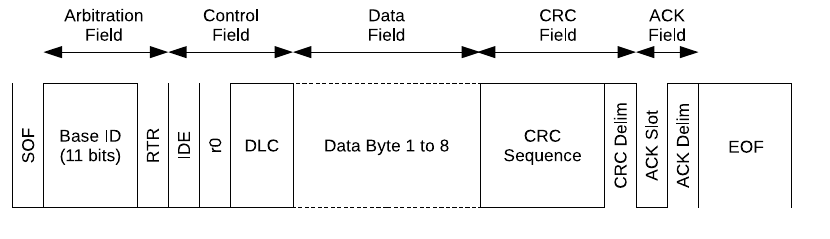
\includegraphics[width=0.8\textwidth]{obrazky/can-frame.png}
            \caption{Struktura datového rámce sběrnice \acs{can}. Převzato z~\cite{esp32-datasheet}}
            \label{fig:obrazky/can-frame.png   }
        \end{figure}
        

    V navrženém systému nese identifikátor zprávy dvě informace. První tři odesílané bity značí typ zprávy. Rozlišena je zpráva určené všem jednotkám (BR -- Broadcast), zpráva od řídicí jednotky k periferiím (TS -- master To Slave), od periferie zpět k řídicí jednotce (TM -- slave To Master) a debug zpráva sloužící k odeslání diagnostických dat nezávisle na ostatní komunikaci. Zbylých 8 bitů pak tvoří adresu jednotky odesílající zprávu (v případě TM) resp. zprávu přijímající (v případě TS). 
    
    \subsection{Adresace}
    Adresy jednotlivých modulů by měly být po startu systému nebo připojení nové jednotky automaticky přiděleny tak, aby nedošlo ke kolizi adres ani v případě připojení několika sensorů stejného typu. Princip adresace spočívá v sérii několika BR zpráv. Po startu systému pošle řídicí jednotka požadavek na adresaci, jako odpověď odešlou jednotky periferíí své unikátní sériové číslo přičemž pouze jedna ze zpráv vyhraje arbitraci. Řídicí jednotka odpoví zprávou, která obsahuje sériové číslo úspěšné jednotky a přidělenou osmibitovou adresu. Následně zopakuje požadavek adresace a odpoví již pouze jednotky bez adresy, po dokončené adresaci pak neodpoví žádná jednotka. Pokud je do běžícího systému připojena nová periferie, odešle sama BR zprávu s požadavkem na přidělení adresy.

    Ačkoliv je tento princip vymyšlen, v rámci prototypu prozatím není implementován a otestován a každý typ periferie má pevně přidělenou adresu, lze tedy připojit pouze jednu periferii stejného typu. V současné chvíli je toto řešení dostačující.



\section{Firmware řídicí jednotky}
    Firma Espressif nabízí pro své mikrokontroléry dva základní frameworky. Oba jsou vyvíjeny jako open-source a jsou tedy také volně dostupné pro jakékoliv použití. Univerzálním řešením vhodným i pro komerční aplikace je ESP-IDF (Espressif Integrated Development Framework). Pro hobby projekty lze využít také Arduino framework, který je taktéž oficiálně podporovaný. Poslední novinkou je pak možnost programování v jazyce Rust namísto klasického C/C++, tento projekt je vytvářen komunitou uživatelů za podpory společnosti Espressif, prozatím ale nebyla oficiálně vydána stabilní verze. 

    V rámci této práce je využit framework ESP-IDF spolu s několika volně dostupnými knihovnami. Toto řešení již obsahuje HAL kód pro práci s periferiemi MCU, není tedy potřeba pracovat přímo s procesorovými registry. Framework má také podporu pro jednoduchý operační systém FreeRTOS, který je rovněž v této práci využit~\cite{espressif-idf}. 

    \subsection{FreeRTOS}
        Systém FreeRTOS umožňuje vytvářet tzv. tasky neboli samostatné procesy které běží z pohledu uživatele paralelně. Jelikož má zvolený mikroprocesor dvě jádra, mohou dva tasky běžet skutečně paralelně, více procesů se pak ve svém běhu střídá a běží tak přerušovaně, dá se říci pseudoparalelně. O tuto režii se stará samotný operační systém a vývojář má několik možností, jak tento proces ovlivnit. V případě vytížení procesoru systém přiděluje čas na základě nastavených priorit a dá přednost tasku s vyšší prioritou, může se tak stát, že některý proces zůstane pozastaven na dlouhou dobu. Při tvorbě kódu je potřeba mít toto na paměti, vhodně zvolit priority tasků a také průběžně sledovat vytížení procesoru jednotlivými tasky.  

        Aby byl kód tzv. thread-safe, tedy bezpečný pro přístup z více vláken, je potřeba ošetřit případy, kdy více tasků pracuje se stejnými daty nebo přistupuje ke stejné periferii mikrokontroléru. K tomuto účelu FreeRTOS nabízí synchronizační objekty jako jsou mutexy, semafory případně fronty. 

    \subsection{Indikace stavu zařízení}
    \label{kap:indikace-stavu-ridici-jednoty}
        Šasi řídicí jednotky je vybaveno adresovatelným barevným \acs{led} páskem sestávajím ze čtyř diod jejichž úkolem je signalizovat uživateli stav zařízení. Jednotlivé stavy spolu s popisem diod jsou zobrazeny na obr.~\ref{fig:stavove-led-mainboard}. Každý task, který je součástí procesu diagnostiky má svou vlastní globální proměnnou do které ukládá svůj stav. Dvakrát za vteřinu se pak spustí jednoduchá diagnostická funkce (běží v rámci vlastního tasku), která jednotlivé stavové proměnné přečte, vyhodnotí celkový stav zařízení a aktualizuje barvu stavových \acs{led}. 
        \begin{figure}[h!]
            \centering
            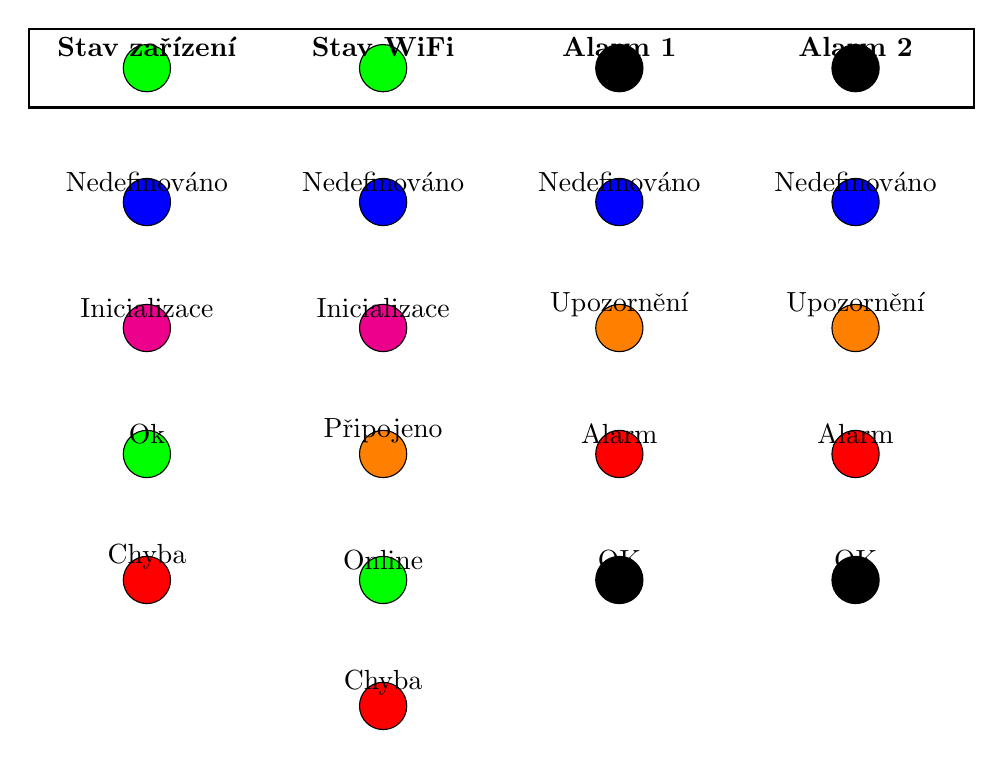
\begin{tikzpicture}
                % Draw a rectangle
                \draw[thick] (0,0) rectangle (3*4,1);
                
                % Draw and fill four colorful circles
                \filldraw[fill=green,draw=black,thin]  (3*0.5, 0.5) circle (0.3) node[align=center,above=0.5] {\textbf{Stav zařízení}};
                \filldraw[fill=green,draw=black,thin]  (3*1.5, 0.5) circle (0.3) node[align=center,above=0.5] {\textbf{Stav WiFi}};
                \filldraw[fill=black,draw=black,thin]  (3*2.5, 0.5) circle (0.3) node[align=center,above=0.5] {\textbf{Alarm 1}};
                \filldraw[fill=black,draw=black,thin]  (3*3.5, 0.5) circle (0.3) node[align=center,above=0.5] {\textbf{Alarm 2}};

                % Draw and fill four colorful circles
                \filldraw[fill=blue,draw=black,thin]    (3*0.5, -1.5*0.8) circle (0.3) node[align=center,above=0.35] {Nedefinováno};
                \filldraw[fill=blue,draw=black,thin]    (3*1.5, -1.5*0.8) circle (0.3) node[align=center,above=0.35] {Nedefinováno};
                \filldraw[fill=blue,draw=black,thin]    (3*2.5, -1.5*0.8) circle (0.3) node[align=center,above=0.35] {Nedefinováno};
                \filldraw[fill=blue,draw=black,thin]  (3*3.5, -1.5*0.8) circle (0.3) node[align=center,above=0.35] {Nedefinováno};

                % Draw and fill four colorful circles
                \filldraw[fill=magenta,draw=black,thin] (3*0.5, -3.5*0.8) circle (0.3) node[align=center,above=0.35] {Inicializace};
                \filldraw[fill=magenta,draw=black,thin] (3*1.5, -3.5*0.8) circle (0.3) node[align=center,above=0.35] {Inicializace};
                \filldraw[fill=orange,draw=black,thin]  (3*2.5, -3.5*0.8) circle (0.3) node[align=center,above=0.35] {Upozornění};
                \filldraw[fill=orange,draw=black,thin]  (3*3.5, -3.5*0.8) circle (0.3) node[align=center,above=0.35] {Upozornění};

                % Draw and fill four colorful circles
                \filldraw[fill=green,draw=black,thin]   (3*0.5, -5.5*0.8) circle (0.3) node[align=center,above=0.35] {Ok};
                \filldraw[fill=orange,draw=black,thin]  (3*1.5, -5.5*0.8) circle (0.3) node[align=center,above=0.35] {Připojeno};
                \filldraw[fill=red,draw=black,thin]   (3*2.5, -5.5*0.8) circle (0.3) node[align=center,above=0.35] {Alarm};
                \filldraw[fill=red,draw=black,thin]  (3*3.5, -5.5*0.8) circle (0.3) node[align=center,above=0.35] {Alarm};

                % Draw and fill four colorful circles
                \filldraw[fill=red,draw=black,thin]     (3*0.5, -7.5*0.8) circle (0.3) node[align=center,above=0.35] {Chyba};
                \filldraw[fill=green,draw=black,thin]   (3*1.5, -7.5*0.8) circle (0.3) node[align=center,above=0.35] {Online};
                \filldraw[fill=black,draw=black,thin]   (3*2.5, -7.5*0.8) circle (0.3) node[align=center,above=0.35] {OK};
                \filldraw[fill=black,draw=black,thin]   (3*3.5, -7.5*0.8) circle (0.3) node[align=center,above=0.35] {OK};

                % Draw and fill four colorful circles
                \filldraw[fill=red,draw=black,thin]     (3*1.5, -9.5*0.8) circle (0.3) node[align=center,above=0.35] {Chyba};
            \end{tikzpicture}
            
            \caption{Stavové \acs{led} řídicí jednotky.}
            \label{fig:stavove-led-mainboard}
        \end{figure}

    \subsection{Popis jednotlivých tasků}
        Řídicí jednotka vykonává současně několik funkcí. Komunikuje s periferiemi skrze sběrnci CAN, ovládá připojená relé a stavové diody. Kromě toho také komunikuje s webovým serverem prostřednictvím WiFi. Jednotlivé úlohy je třeba vykonávat periodicky, ovšem každou s jinou prioritou. Kód je proto rozdělen do několika tasků podle své funkce a priority. 

        K synchronizaci tasků jsou využity binární semafory. K převzetí semaforu ve {FreeRTOS} slouží funkce \texttt{xSemaphoreTake( xSemaphore, xBlockTime )}. Na řádku s touto funkcí kód čeká až do přijetí semaforu odeslaného jiným taskem nebo do vypršení času stanoveného druhým parametrem. 

        Každý z tasků začíná inicializací, kdy se jednorázově nastaví potřebné proměnné. Dále pokračuje nekonečnou smyčkou přerušenou vždy čekáním na semafor nebo neblokujícím zpožděním za pomocí funkce \texttt{vTaskDelay( const TickType\_t xTicksToDelay )}.

        % \begin{lstlisting}[language={[LaTeX]TeX}]
        %     \section{Balíček lstlistings}
        %     Pro vysázení zdrojových souborů je možné použít
        %         balíček \href{https://www.ctan.org/pkg/listings}%
        %         {\texttt{listings}}.
        %     Balíček zavádí nové prostředí \texttt{lstlisting} pro
        %         sazbu zdrojových kódů.
        %     \end{lstlisting}
        
        \subsubsection{Kontrolní proces -- \texttt{control\_task}}
            Jedná se o hlavní task programu co se týče samotného algoritmu. Na začátku běhu ve vhodném pořadí spustí ostatní tasky a provede vlastní inicializaci. Je spuštěna adresace zařízení na sběrnici CAN a od připojených periferií následně vyžádána informace o jejich typu, sériovém čísle a současnému stavu. Z perzistentní paměti flash je na základě sériového čísla načtena konfigurace jednotlivých modulů a samotného systému. 

            Ve smyčce je následně pravidelně prováděn sled několika operací. Pokud je to potřeba, dojde ke stažení nové konfigurace ze serveru, aktualizaci odpovídajích proměnných i paměti flash.  O nutnosti této operace rozhoduje \texttt{wifi\_task}.

            Dále jsou obslouženy periferie na sběrnici. Je vyžádán jejich status a dle typu také senzorická a provozní data. 

            Na základě konfigurace systému, získaných dat a reálného času je odeslán požadavek odpovídajícím akčím členům a aktualizován stav relé. Také je zpracován případný alarm, který je následně jiným taskem signalizován prostřednictvím stavových diod. 

            Dle nastavené periody jsou data získaná ze senzorů také odeslána na webový server.

        \subsubsection{Obsluha WiFi --  \texttt{wifi\_task}}
            V inicializační fázi tohoto tasku je vznešen požadavek na připojení k síti WiFi. V případě selhání nebo pozdějšího odpojení je pokus automaticky opakován. 
            
            V nekonečné smyčce pak task periodicky kontroluje dostupnost internetového připojení, dotazuje se serveru na poslední dostupnou verzi konfigurace a aktualizuje údaj o reálném čase (ten je následně uchován vnitřním \acs{rtc} časovačem mikrokontroléru).

        \subsubsection{Obsluha sběrnice CAN --  \texttt{can\_bus\_task}}
            Inicializuje potřebné GPIO piny a připraví potřebné proměnné. Ve smyčce pak pravidelně kontroluje příchozí zprávy na sběrnici (zejména typu Broadcast, které mohou být odeslány periferiemi bez vyzvání). Příchozí zprávy filtruje a pomocí front předává dalším taskům. Na začátku vždy čeká na kontrolní semafor značící požadavek na vyčtení sběrnice. Pokud není vyslán požadavek, čekání na semafor vyprší a sběrnice je zkontrolována s danou periodou.

            \subsubsection{Obsluha WiFi --  \texttt{wifi\_task}}
            V inicializační fázi tohoto tasku je vznešen požadavek na připojení k síti WiFi. V případě selhání nebo pozdějšího odpojení je pokus automaticky opakován. 
            
            V nekonečné smyčce pak task periodicky kontroluje dostupnost internetového připojení, dotazuje se serveru na poslední dostupnou verzi konfigurace a aktualizuje údaj o reálném čase (ten je následně uchován vnitřním \acs{rtc} časovačem mikrokontroléru).

        \subsubsection{Indikace stavu --  \texttt{status\_update\_task}}
            Zpracovává stavové proměnné ostatních tasků a na základě těchto dat vyhodnocuje stav zařízení. Tento stav následně indikuje za pomoci stavových diod, jak bylo popsáno v kapitole~\ref{kap:indikace-stavu-ridici-jednoty}.



\section{Firmware periferií}
    Jak bylo popsáno v kapitole~\ref{sec:modul-periferie}, všechny periferie mají stejné jádro. Ve všech pracuje stejný mikrokontrolér (PIC18F26), stejným způsobem pracují se sběrnicí CAN a také část příkazů na sběrnici je všem periferiím společná. Rozdíl mezi periferiemi je daný pouze připojenými sensory. Ty vyžadují vždy specifické nastavení vstupních a výstupních pinů, zpracování dat a jejich odeslání skrze sběrnici CAN. 

    Tato struktura je replikována také ve zdrojovém kódu. Pro všechny periferie existuje společný projekt, kdy základní kód zůstává vždy stejný. Pro sestavení a nahrání programu do konkrétního modulu je potřeba upravit hlavičkový soubor \texttt{device\_type.h}. Tento soubor nastaví typ zařízení a následně za pomoci preprocesorových direktiv vloží do projektu pouze odpovídající knihovny. Výňatek z tohoto souboru je zde uveden jako výpis~\ref{lst:devicetype}. Stejným principem je kód větven na všech místech, kde je toto potřeba. 

    Program sestává ze dvou hlavních částí. Nejprve je to fáze incializace, kdy dojde k nastavení potřebných registrů a proměnných. Poté zařízení vstupuje do nekonečné smyčky. V té jsou periodicky vyčítána data z připojených senzorů resp. ovládány akční členy.  Příchozí zprávy na sběrnici CAN vyvolají vždy přerušení, zpracovávají se tedy mimo hlavní smyčku programu. 

\clearpage % TODO zarovnat dle zbytku
\begin{lstlisting}[frame=single,caption={Část souboru \texttt{device\_type.h} sloužící k výběru typu cílené periferie.},label=lst:devicetype,basicstyle=\ttfamily\small, keywordstyle=\color{black}\bfseries\underbar,]
#ifndef DEVICE_TYPE_H
#define	DEVICE_TYPE_H

// soubor procesoru PIC
#include <xc.h>   

// knihovna sdílená s řídicí jednotkou
#include "../shared/common_types.h" 

// Výběr jedné z hodnot definovaných v common_types.h
#define DEVICE_TYPE     DEVICE_TYPE_WATER_LEVEL_SENSOR

...

// Hlavičkové soubory specifické dle typu periferie
#if DEVICE_TYPE == DEVICE_TYPE_LED_BOARD
    #include  "led_board_driver/led_board_driver.h"
#elif DEVICE_TYPE == DEVICE_TYPE_TEMP_SENSOR
    #include "temp_sensor_driver/temp_sensor_driver.h"
#elif DEVICE_TYPE == DEVICE_TYPE_WATER_LEVEL_SENSOR
    #include "water_level_driver/water_level_driver.h"
...
#else
    #error "Not supported DEVICE_TYPE"
#endif
#endif	/* DEVICE_TYPE_H */
\end{lstlisting}

\subsection{Zpracování příkazů CAN}
    Jako základ je využit kód vytvořený modulem Microchip Code Configurator. Jedná se o užitečný nástroj, který předpřipraví kód nutný k nastavení konkrétních registrů. Také obsahuje funkce úrovně HAL, aby nebylo nutné dále pracovat přímo s registry. Vygenerovaý kód je přitom krátký a snadno čitelný. Veškeré generované nastavení bylo následně kontrolováno s katalogovým listem procesoru a v případě potřeby upraveno. 

    Na rozdíl od procesoru řídicí jednotky, PIC18F26 obsahuje v periferii CAN až 11 různých filtrů příchozích zpráv~\cite{PIC18F26Q83}. Již na úrovni hardwaru jsou tak zprávy rozděleny dle typu. Zprávy určené periferiím (TS - To Slave) jsou řazeny do jedné fronty, zprávy určené všem (BR - Broadcast) pak do druhé fronty. Ostatní zprávy nejsou zpracovány vůbec. Při přijetí zprávy je vyvoláno přerušení a kód přečte zprávu z dané fronty. Pokud je to potřeba, odešle vlastní zprávu jako odpověď. První bajt datového pole zprávy vždy identifikuje daný příkaz. 

\subsection{Smyčka programu}
    Jelikož zpracování příkazů ze sběrnice CAN probíhá vždy jako obsluha přerušení, samotná smyčka programu je velmi jednoduchá.  V případě sensorů ji lze rozdělit do tří kroků. Nejprve jsou vyčtena surová data ze sensorů a uložena do vhodných proměnných. Ve druhém kroku jsou data zpracována -- je vyhodnocena jejich správnost, provedena korekce nebo přepočet, případně jsou data průměrována z více opakování měření. Ve třetím kroku jsou zpracovaná data uložena do globální promměnné. Pokud přišel po sběrnici CAN požadavek na odeslání dat, jsou mu předána tato data. 

    Na konci smyčky je pak vždy vyhodnocen stav zařízení a opět uložen do globální proměnné.

    Přesný průbeh jednotlivých kroků programové smyčky se liší v závislosti na typu periferie a byl upravován průběžně k dosažení optimální funkce jednotlivých sensorů.




\section{Webové rozhraní}
    Aby bylo možné systém konfigurovat a monitorovat, bylo zapotřebí navrhnout a vytvořit webové rozhraní. Důležitým krokem v rozhodování byla volba, zda bude \acs{mcu} řídicí jednotky sloužit přímo jako webový server nebo pouze jako klient. První scénář klade podstatně vyšší nároky na zatížení a paměť \acs{mcu}, výhodou je ale velmi jednoduchý systém, který funguje samostetně bez nutnosti externího serveru případně také bez připojení k internetu (ESP32 může sloužit přímo jako přístupový bod). Výhodou druhé varianty je větší flexibilita, externí server má nesrovnatelně vyšší výkon a kapacitu úložiště a umožní tak tvorbu mnohem komplexnější webové stránky, která bude (v případě připojení serveru do internetu) dostupná odkudkoliv. Server zároveň může ukládat měřená data a ta tedy budou dostupná i v případě, že samotné zařízení je mimo provoz nebo není připojeno k síti.

    V rámci realizace této práce byla zvolena varianta externího serveru. Jádro vytvořené webové aplikace tvoří program v jazyce PHP, který zpracovává jak požadavky uživatele, tak i samotného zařízení. Na pozadí dále běží databázový server s otevřeným systémem MySQL, sloužící k uchování provozních dat. V databázi jsou uloženy údaje o uživatelích, systémech akvárií (tedy řídicí jednotka a k ní připojené periferie) a jejich konfiguraci. Také jsou zde ukládána data ze senzorů. V záznamu odpovídajícímu danému systému akvária je uložen číselný údaj o aktuální verzi konfigurace. Pokud uživatel změní některé nastavení, toto číslo se inkrementuje. Na verzi konfigurace se zařízení pravidelně dotazuje a v případě změny si následně stáhne zažádá o celou novou konfiguraci.

    \subsection{API rozhraní -- komunikace z pohledu zařízení}
    Zařízení komunikuje s webem pomocí aplikačního rozhraní (API), které tvoří nenáročný způsob komunikace využívající formát JSON. Jednotlivé adresy API rozhraní jsou přehledně popsány v tab.~\ref{TODO}. 

    \begin{table}[h]
        \centering
        \caption{Přehled periferií.}
        \label{tab:prehled-periferii}
        \begin{tabular}{|l|l|l|l|}
            \hline
            Adresa & Funkce & Odchozí data\(^{*}\)  & Příchozí data\(^{*}\)  \\ \hline\hline
           
            /ping & Kontrola dostupnosti & - & -  \\ \hline
            /ping?SN= & Kontrola konfigurace & Sériové číslo & Verze konfigurace  \\ \hline
            /config/get?SN= & Stažení konfigurace & Sériové číslo & Plná konfigurace  \\ \hline
            /data/add & Odeslání dat & Provozní data & -  \\ \hline
            /data/view & Načtení dat & - & Data pro zobrazení na webu  \\ \hline
                            %     & S &  &  & A  \\ \hline
                            %     & S &  &  & A  \\ \hline
                            %     & S &  &  & A  \\ \hline
                            %     & S &  &  & A  \\ \hline
                            %     & S &  &  & A  \\ \hline
                            %     & S &  &  & A  \\ \hline
                            %     & S &  &  & A  \\ \hline
            \end{tabular}
            \begin{tabular}{c}
                \(^{*}\)Z pohledu  řídicí jednotky.
            \end{tabular}   
    \end{table}

    \subsection{Uživatelská aplikace}
        Z pohledu uživatele je možnost se na webu registrovat a přihlásit. Teprve po přihlášení je zobrazeno grafické menu. Webová aplikace slouží dvěma hlavním funkcím, kterým odpovídají také položky menu. 
        
        První položkou je zobrazení stavu zařízení. Kliknutí na odkaz přivede uživatele na podstránku zobrazující grafy všech dostupných dat jeho akvarijního systému. V grafech je v tuto chvíli zobrazeno vždy 100 posledních hodnot. 

        \begin{figure}[h!]
            \centering
            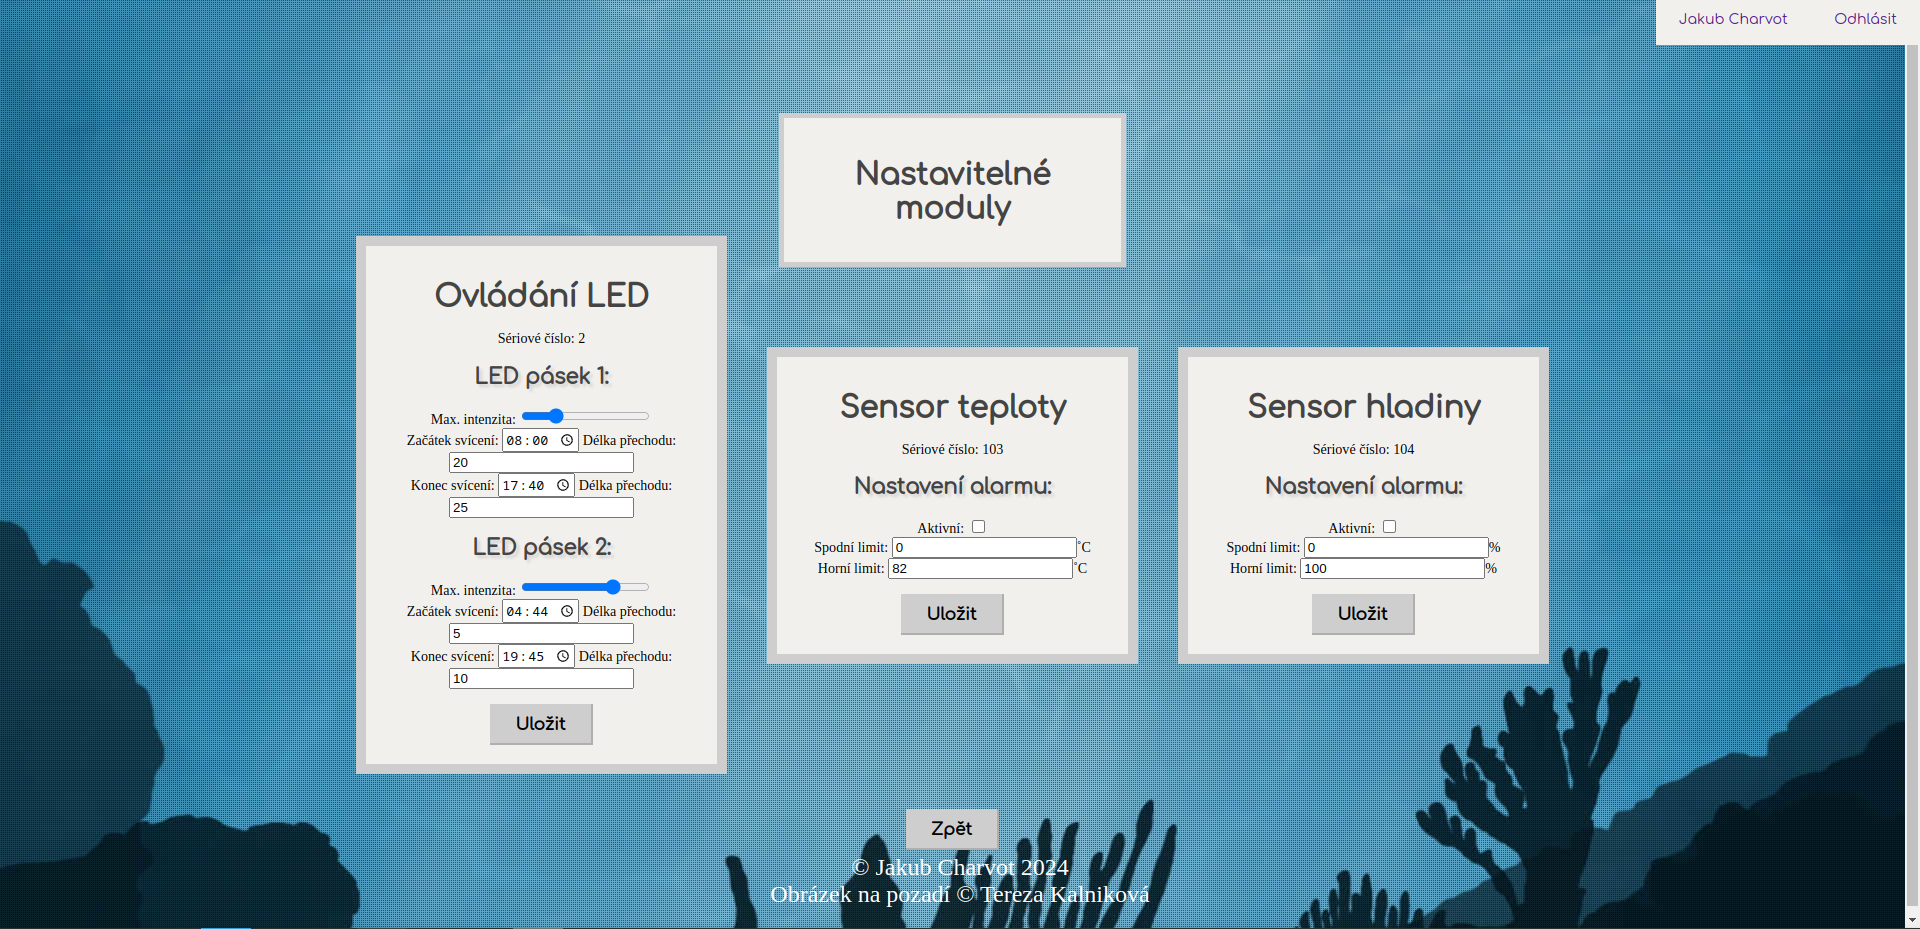
\includegraphics[width=\textwidth]{obrazky/web.png}
            \caption{Ukázka jedné ze stránek webové aplikace.}
            \label{fig:obrazky-web.png}
        \end{figure}
        

        Druhou položka je zde nazvaná jako \uv{Scénáře} a nachází se v ní konfigurace systému a nastavení jednotlivých modulů. Pro sensory lze nastavit úrovně, které má systém vyhodnotit jako alarmující. Pro každou síťovou zásuvku je pak možné přepnout mezi dvěma režimi. V manuálním režimu uživatel přímo nastaví sepnutí nebo rozepnutí zásuvky, druhým režimeme je pak časovač, kdy lze nastavit pravidelné časy vypnutí a zapnutí.

        Pro představu o vzhledu webu je zde přiložen obr.~\ref{TODO screenshot}, v elektronické příloze je pak snímků více.